\documentclass{jarticle}

\usepackage{geometry}
\usepackage{cite}
\usepackage[dvipdfmx]{graphicx}
\usepackage{here}
\usepackage{amsmath}
\usepackage{amsfonts}
\bibliographystyle{junsrt} %参考文献出力スタイル


\geometry{left = 20mm, right = 20mm}
\title{非定常時系列の教師なしクラスタリング:位相的データ解析による分析}
\author{黒木 裕鷹}
\date{2018年4月27日}

\begin{document}
\maketitle
\section{はじめに}
膨大な特徴量をもつ高次元データ解析において,どのように高次元の特徴量を低次元で表現するのかは重要な研究課題である.近年,位相的データ解析による高次元データ解析が盛んに提案されており,複雑な高次元データの位相的情報を可視化する手法として注目を集めている.

データの位相構造とは,

位相的データ解析を利用した,高次元データ解析の研究対象としては***や***による??解析や***による金融市場分析,***によるマーケティングの応用や***などがある.これらの研究では,

現在,世界の様々な工場では産業用ロボットが用いられている.そのような工場では,重量物の運搬を必要としたり,霧散している粉塵を吸い込んだりする危険性など,人間には負担の大きい作業の割合が多い.
産業用ロボットはこのような安全性の問題を解決するだけでなく,経済性や効率性においてもメリットがある.
しかし同時にロボットには故障のリスクがあり,ただひとつのロボットの故障が生産ライン全体に影響を及ぼし得る.
故障を未然に回避するためにはメンテナンスなどの保守作業を行うことが重要であるが,メンテナンスや部品交換にも費用や時間などコストがかかるため,適切なタイミングで行われることが望ましい.


自動車メーカーのMでは,生産ラインで使用するアームロボットの故障を未然に防ぐため,その減速機の交換を経験に基づくタイミングで行っている.
交換のタイミングが遅すぎれば故障を招くが,早すぎても交換に時間がかかる分パフォーマンスが低下することとなる.
本調査では,ロボットアームをモニタリングした振動のセンサーデータを用い,減速機交換前後のデータに明確な違いがあるかどうかを調査した.
ロボットの故障により生産ラインを止めることはあってはならないため,故障直前のデータは得ることが出来ないことに留意しなければならず,教師無し学習によるクラスタリングを行うことを目的とした.


Mより提供されたデータは一つのロボットアームにつき,減速機交換前後それぞれで5秒間の計測を10回行った1次元の振動データである.
ロボットアームはそれぞれ挙動が異なるため,その主要な振動はアームごとに異なっている.
また,各アームの行動1セットは5秒間ではないため,各計測ごとにより行動セットの中の計測する部分が異なっている.

クラスタ分析では,クラスタリングされる対象間の類似度もしくは非類似度が必要である.
時系列を対象としたクラスタリングにおいて,最も広く使用されている尺度はユークリッド距離,Dynamic Time Warping(DTW)\cite{Berndt1996},CORT\cite{Chouakria2007}などである.
DTWは2つの時系列データの時刻を$t_i$, $t_j$とすると,$t_i,t_j$全ての組の誤差を計算し,それらの合計が最小になるような経路を求めるアルゴリズムである.
そのため,DTWは二つの系列の周期や長さが異なる場合でも非類似度を算出することができる.
DTWにより挙動の計測開始時点が異なる問題は多少解決されるが,振動の主な挙動はアームによって異なるため,減速機交換前後の差異はクラスタリングの結果に表れない.
また,未知音源分離で用いられる独立成分分析(ICA)は主要な振動と微細な振動を分けることを可能にするかもしれないが,同時点の複数観測を必要とするため本データには適用することはできない.
つまり時系列の同時性を利用することなく,かつアームごとに異なる主要な振動に影響されない特徴量によって教師無し学習を行うことが課題である.


本調査では,以上のような課題を解決するため,データの位相的な特徴に注目した.
近年着目されているTopological Data Analysis(TDA)は複雑なデータを扱う上で強力であり,パーシステント・ホモロジー\cite{Edelsbrunner2002}とその表現であるパーシステント・ダイアグラム\cite{Otter2017}をはじめとするその手法はデータの位相的特徴を抽出し,新しい知見を与える.
またTDAの分野で広く行われているように,時間遅れ座標を用いて時系列を多次元に埋め込むことで位相的特徴を抽出する足掛かりとした.
時間遅れ座標による埋め込みはダイナミカルシステムの分野で,状態空間の復元を目的に広く用いられている.
パーシステント・ダイアグラムを比較するためにWasserstein距離\cite{Mileyko2011}がしばしば用いられるが,本調査で扱うようなデータでは計算量の観点で現実的ではない.
また,\cite{Umeda2017}の提案するBetti sequenceはデータの位相情報を1次元の系列として要約する.
そこで本調査では,観測の上述した観測の長さや観測開始時点が異なる問題を解決するためにセンサーデータの位相情報を要約したBetti sequenceをもとめ,DTWに基づく全結合型階層的クラスタリングを行うことにより,減速機交換前後の振動を分析した.


本レポートの構成は次のようである.
まず2節では本調査で使用したTDAの手法やクラスタリング手法について述べ,3節では実際のデータ解析とその結果を示す.
4節では考察を行うと共に今後の展望について触れる.

\section{Topological Data Analysis(TDA) と時系列クラスタリング}
トポロジーを用いてデータの情報を抽出するものであり,その主要な手法はmapper\cite{Singh2007}とパーシステント・ホモロジー\cite{Edelsbrunner2002}である.
これらはノイズを含む複雑なデータセットから何か新たな知見を得る目的でしばしば用いられてきた.
本調査ではパーシステント・ホモロジーを利用する.

\subsection{パーシステント・ホモロジー}
距離空間$(M, d_M)$の有限点集合を$X$,$X$を中心とした半径$r$の級の和集合を$B(X;r):=\bigcup_{i=1}^n B(x_i;r)$とする.
ただし,$B(x;r) =\{y \in M | d_M(x,y) \leq r\}$とする.
級の和集合を半径パラメータ$r$で集めた集合$\mathbb B(X):=\{B(X;r)\}_{r\geq 0}$をここでは$X$のフィルトレーションという.
$r\leq a$ならば包含関係$B(X;r)\subset B(X;a)$があるため,ホモロジー群間の射$u_r^a : H_q(B(X;r))\rightarrow H_q(B(X;a)) $を包含写像から誘導する.
このとき,ホモロジー群の系列
$$
H_q(\mathbb B(X)):\dots\rightarrow H_q(B(X;r))\overset{u_a^b}{\rightarrow} H_q(B(X;a))\rightarrow\dots (r\leq a)
$$
を$X$の$q$次元パーシステントホモロジーという.
パーシステントホモロジー体係数多項式環や$A_n$型箙の表現などの言葉で解釈することが出来,分解定理により適切な区間表現$\mathbb I[b_i, d_i] $を通じて
$$
H_q(\mathbb B(X))\cong\oplus\mathbb I[b_i,d_i] (b_i\leq d_i)
$$
と分解される.これをユークリッド空間$\mathbf R^2$内に表示した多重集合
$$
D_q(X):= \{(b_i,d_i) | i \in I\}
$$
を$X$の$q$次元パーシステント・ダイアグラムという.
パーシステント・ダイアグラムの元$(b_i, d_i)$はホモロジーの生成元の発生時間(Birth time)を$b_i$,消滅時間(Death time)を$d_i$と記録しているものと解釈できる.

$q$次のパーシステント・ダイアグラムは2次元の散布図として表され,その解釈や扱いが困難である.
そのため,様々なダイアグラムの要約が提案されてきた.
最も単純なものが最大パーシステンスであり,$\text{max}_i(b_i - d_i)$
で表される.

\subsection{パーシステント・バーコード}
前節で定義したダイアグラム$D_q(X)$のホモロジー$i$に対して,次の$s_i(r)$を定義する.
$$
s_i(r) = 
\begin{cases}
1 & (b_i \leq r \leq d_i)\\
0 & otherwise
\end{cases}
$$
$s_i(r)$を並べてプロットしたものをパーシステント・バーコードという.

また,\cite{Umeda2017}はバーコードを単純に扱い,機械学習の枠組みで扱いやすくするために次で提案されるBetti sequence,$BS(X)$を提案している.
$$
BS(X) = \sum_i s_i(r)
$$
Betti sequenceは半径$r$のときにいくつのホモロジーが存在しているかを表す1次元の系列となる.

\subsection{1次元時系列データに対するTDA}
時系列から複数次元の有限点集合を構成する方法として,遅れ時間座標を利用した埋め込み(embedding)がある.
埋め込みはアトラクタを再構成するために非線形ダイナミカルシステムの分野で盛んに利用されている.
長さ$N$の時系列$x_1, x_2, \dots , x_T$から適当な遅れ時間$\tau$ごとの$d$個の測定値を取り出し$V(t) = (x(t), x(t+\tau), \dots, x(t + d - 1)),\ (t = 1,2,\dots, T)$の$d$次元有限点集合を得る.
この有限点集合が元の$k$次元力学系の埋め込みになるための十分条件として,$d\geq 2k+1$(ターケンスの埋め込み定理)が知られている.

また,有限点集合の次元$d$が大きくなったときに$\mathbb R^d$の$n$個の点集合のドロネー三角形分割の計算量は$\mathcal O(n^{\frac{[d]}{2}})$になりうる\cite{Amenta2007}, \cite{Attali2003}.
そこで,位相情報を保持しながら計算を簡略化するため,十分多次元に埋め込んだ後主成分分析により3次元に次元削減するアプローチが提案されている\cite{Truong2017}.


\subsection{時系列クラスタリング}
時系列間の非類似度を算出する際,用いられているのが\cite{Berndt1996}で提案されたDynamic Time Warping(DTW)である.
DTWは三角不等式を満たさないため距離ではないが,比較的少ない計算量で要素数の異なる系列同士の距離のような量を求める手法である.

また本調査ではDTWに基づき,完全連結方による階層型クラスタリングを行った.
完全連結法とは,クラスタ間で最も類似度が低いデータ間の距離をクラスタ間の距離にする方法である.







\section{データ解析}

\subsection{データの概観}
本調査では,自動車メーカーMの産業用ロボットアームの振動データを扱う.
15種類のロボットアームに対し,減速機を交換する前と交換した後をそれぞれ10回モニタリングした合計300系列のデータである.
計測の基本単位は100ミリ秒であり,計測の長さは5秒間である.ロボットアーム15種類の減速機交換前後のデータのそれぞれ10回分の観測をつなぎ合わせ,以下の図\ref{fig:ts}に示した.
このように,いずれのロボットアームにおいてもその時系列は明らか非線形構造を持つと同時に交換前後の系列は似通っており,アームごとの挙動が主要な振動として現れていることがわかる.
減速機交換前後の特徴を目視で判断することは出来ない.
さらに交換前後で計測開始時間が異なるものもあり,単純な比較が難しいことがわかる.
10回の観測をつなぎ合わせたが,系列は概ね周期的になっている.
しかし一部に周期的でなかったり,交換前後で明らかに異なった振動をしている系列が見て取れる.
\begin{figure}[htbp]
\begin{center}
	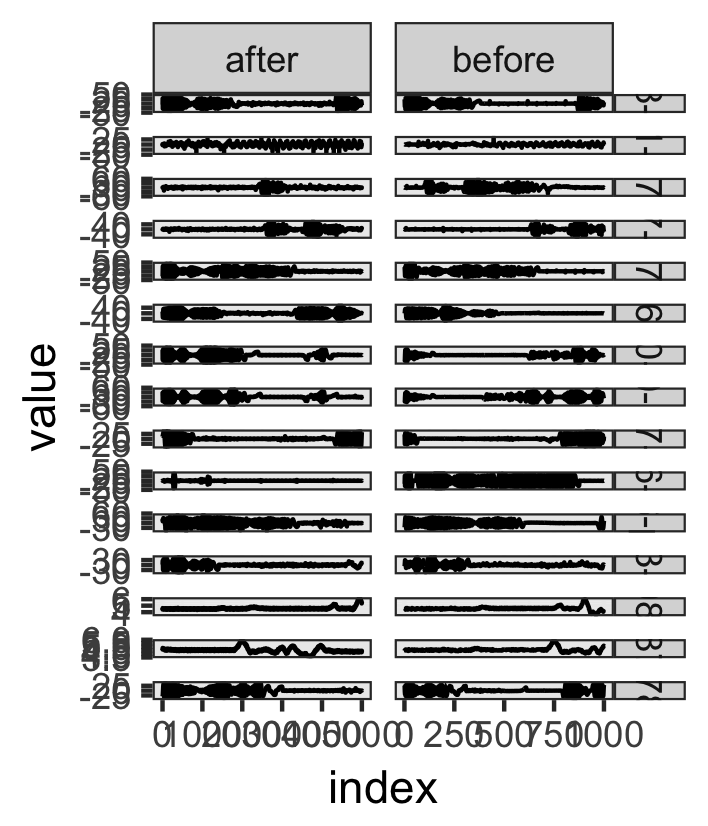
\includegraphics[width=12cm]{fig/ts.png}	
	\caption{センサーデータの時系列プロット\label{fig:ts}}
\end{center}
\end{figure}

\subsection{データの位相的特徴}
ロボットアームによる振動のスケールを調整するため,以下の分析は予め全系列を標準化した上で行った.
1次元の振動時系列から位相情報を取り出すために,遅れ時間座標への埋め込みを行った.
その際,遅れ時間単位は$\tau = 1$とした.
またロボットアームの構造や状態変数の数が明らかでないことから,埋め込み次元にはロボットアームが3次元であることを考慮し,ターケンスの埋め込み定理を参考に$d = 3\times2 + 1 = 7$とした.
さらに\cite{Truong2017}で提案されているように主成分分析を用い第3主成分までを取り出し3次元の有限点集合を抽出した.
アルファ複体のフィルトレーションを用いて抽出した点集合の$0,1,2$次元パーシステント・ホモロジーを計算した.
またその要約として各次元のBetti sequenceを計算し,以下の図\ref{fig:betti1}, \ref{fig:betti2}に示した

\begin{figure}[htbp]
\begin{center}
	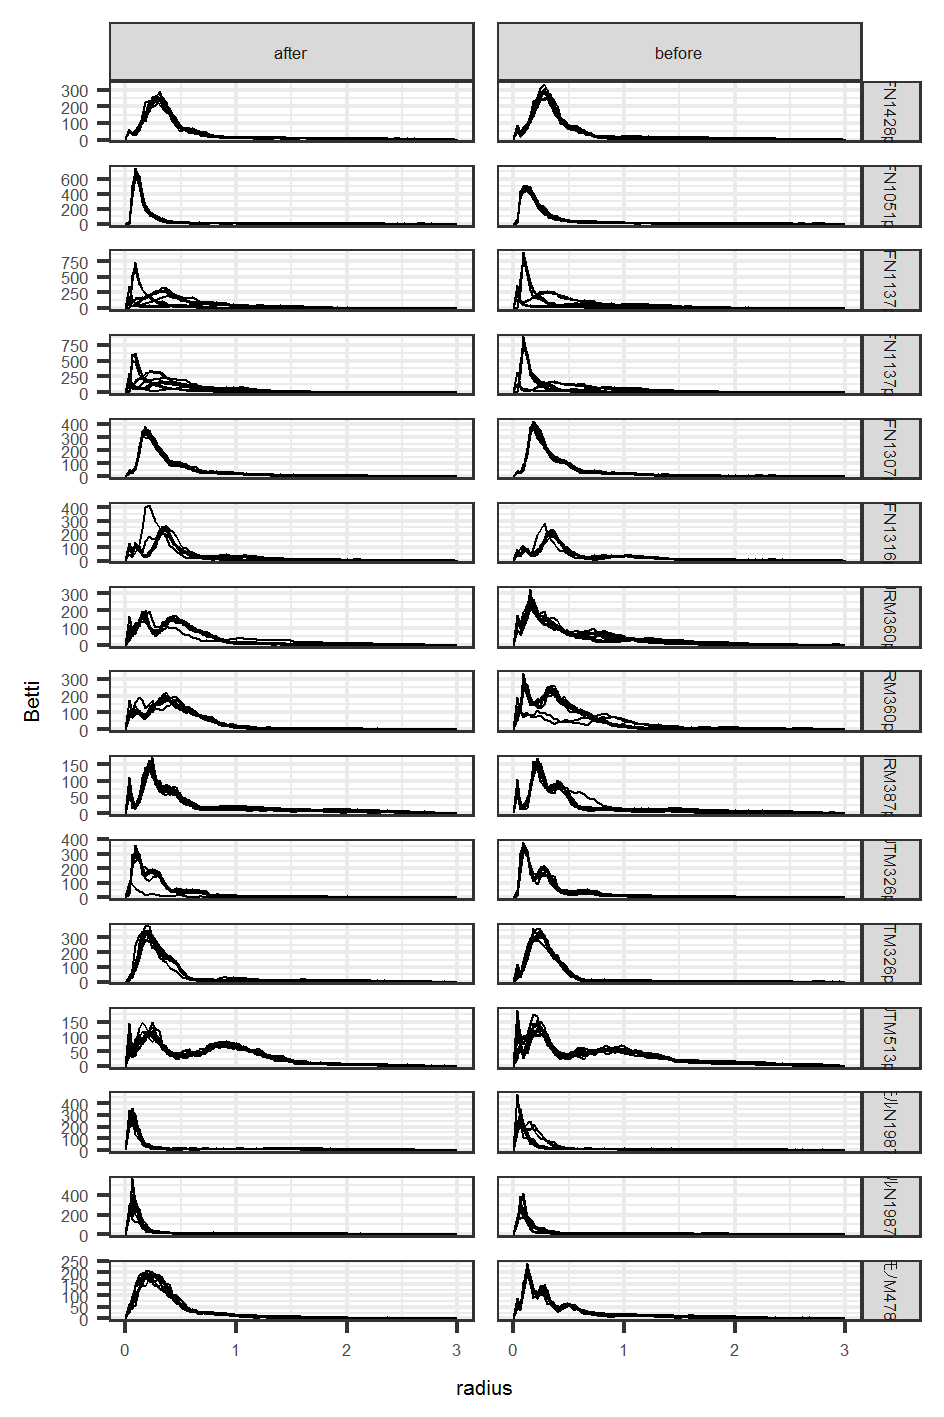
\includegraphics[width=11cm]{fig/betti_1.png}	
	\caption{1次のBetti sequence}\label{fig:betti1}
\end{center}
\end{figure}

\begin{figure}[htbp]
\begin{center}
	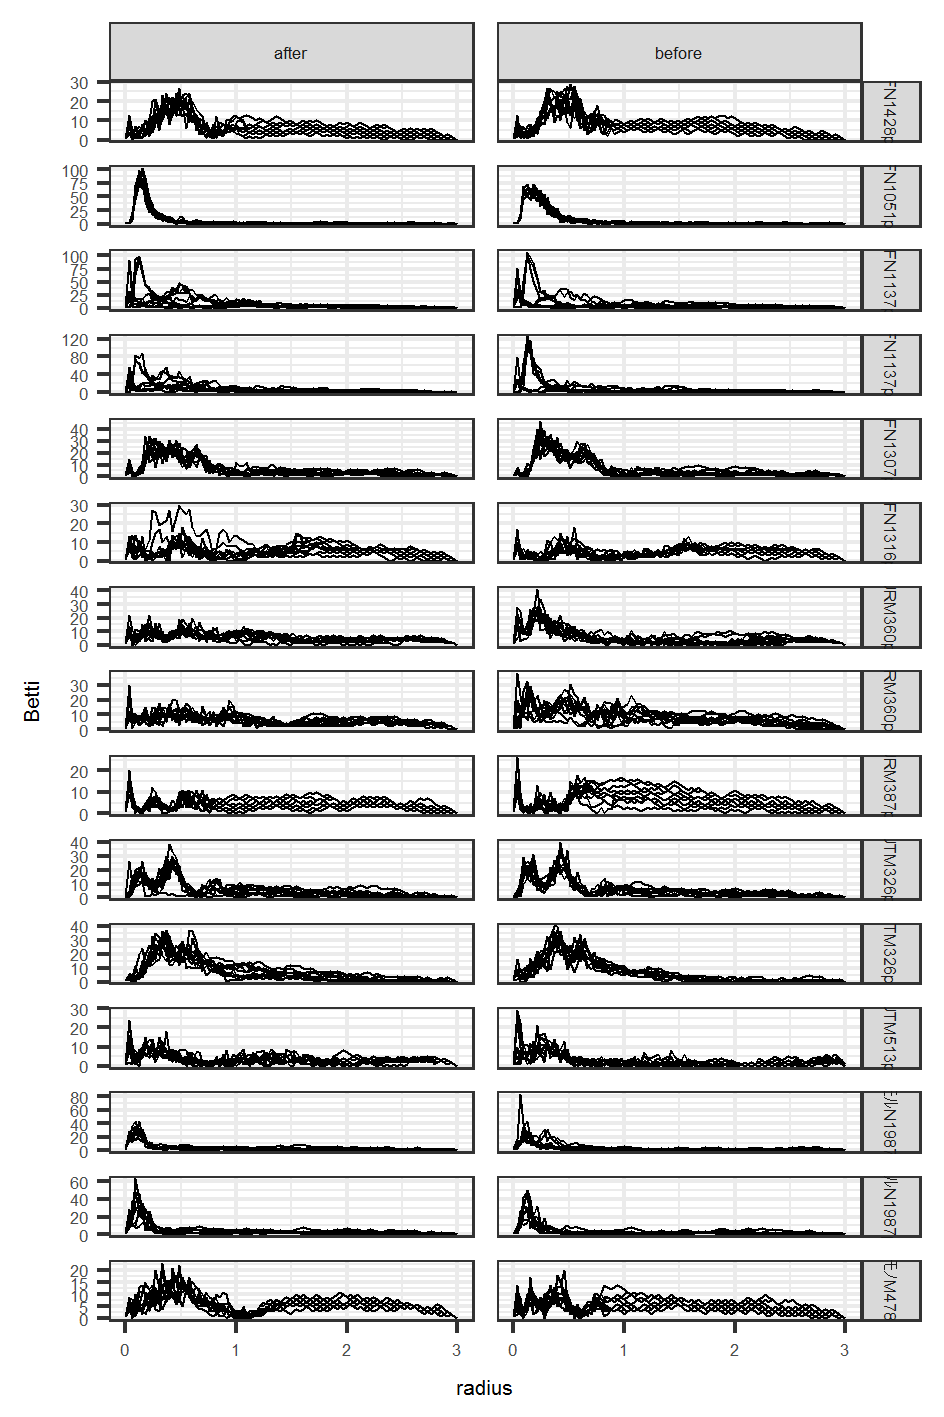
\includegraphics[width=11cm]{fig/betti_2.png}	
	\caption{2次のBetti sequence}\label{fig:betti2}
\end{center}
\end{figure}

図\ref{fig:betti1}, \ref{fig:betti2}より,ほとんどのロボットアームでBetti sequenceが似通っていることがわかる.
また,2次のBetti sequenceは1次のものに比べて観測ごとのばらつきが大きくなっていることが見て取れる.

\subsection{DWTに基づいた時系列クラスタリング}

ロボットアームごとに減速機交換前10系列,交換後10系列の計20系列をクラスタリングすることを考える.
観測ごとのばらつきが少ない1次のベッチ数をもとにDTWを比類似度とした階層的クラスタリングを行った.
クラスター間の距離は完全連結法を用いて算出した.
そのデンドログラムを図\ref{fig:dendro1}から図\ref{fig:dendro15}に示した.

図\ref{fig:dendro1}から図\ref{fig:dendro15}より,いくつかのロボットアームでは明確に減速機交換前後のクラスタが構成できたことが分かる.
またそうでないアームでも細かい部分では減速機交換前後のクラスタができていることが分かる.

\begin{figure}[H]
	\begin{center}
		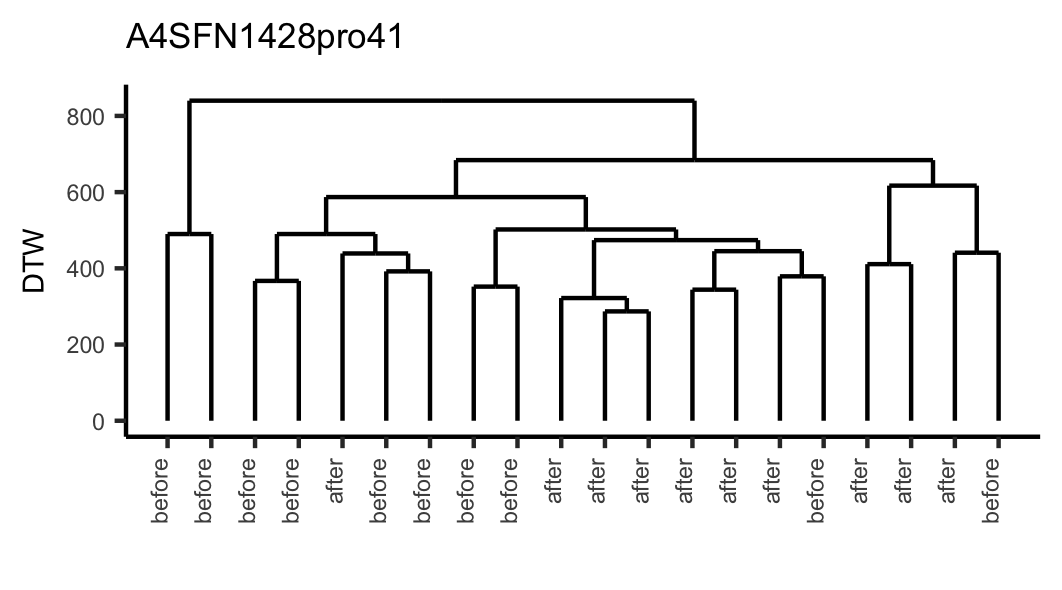
\includegraphics[width=15cm]{fig/dendro_1.png}
		\caption{デンドログラム1}
		\label{fig:dendro1}
	\end{center}
\end{figure}
\begin{figure}[H]
	\begin{center}
		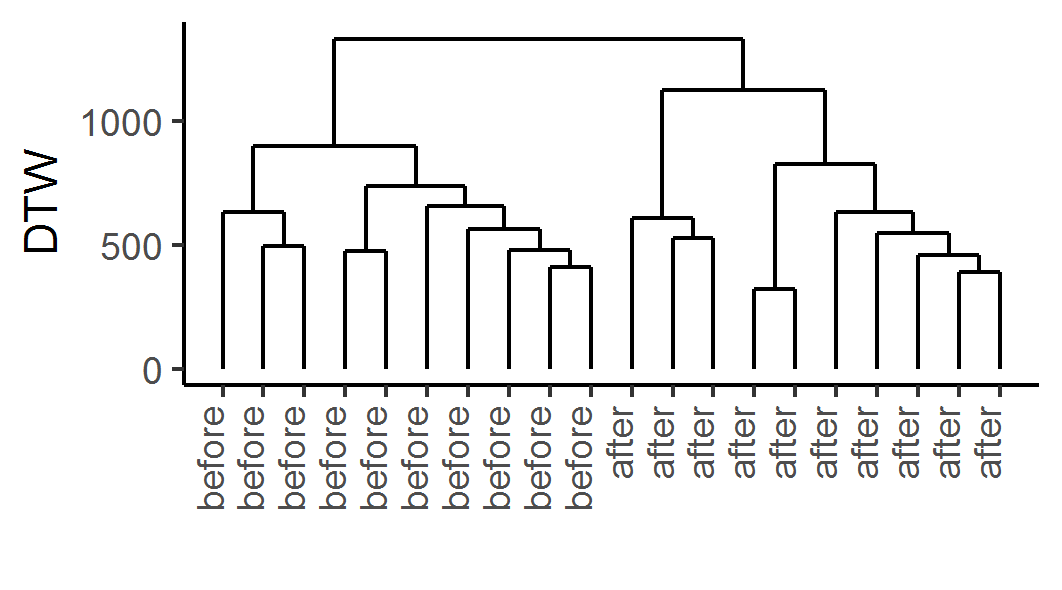
\includegraphics[width=15cm]{fig/dendro_2.png}
		\caption{デンドログラム2}
		\label{fig:dendro2}
	\end{center}
\end{figure}
\begin{figure}[H]
	\begin{center}
		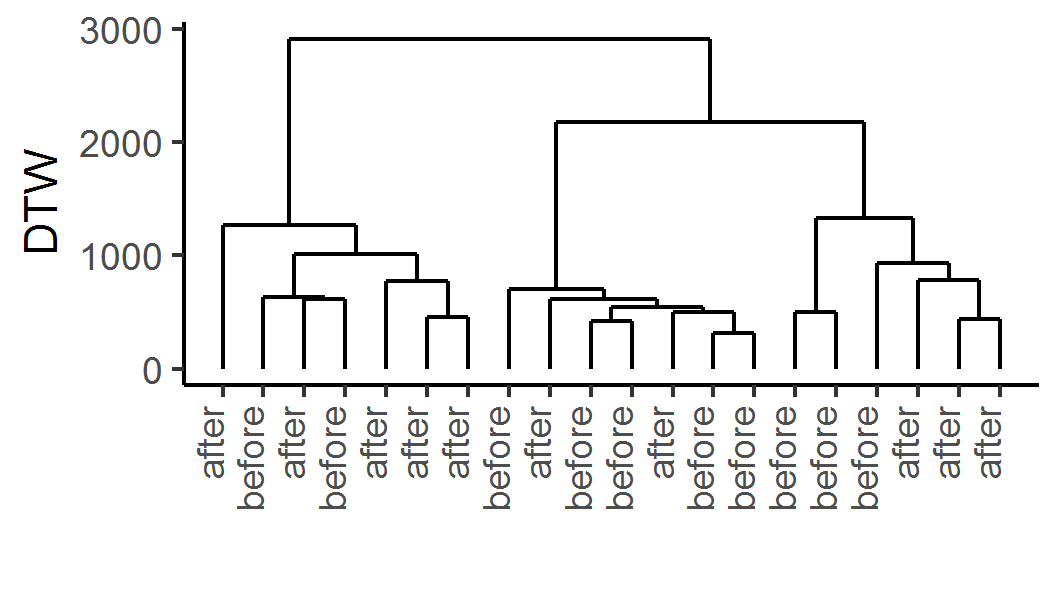
\includegraphics[width=15cm]{fig/dendro_3.png}
		\caption{デンドログラム3}
		\label{fig:dendro3}
	\end{center}
\end{figure}
\begin{figure}[H]
	\begin{center}
		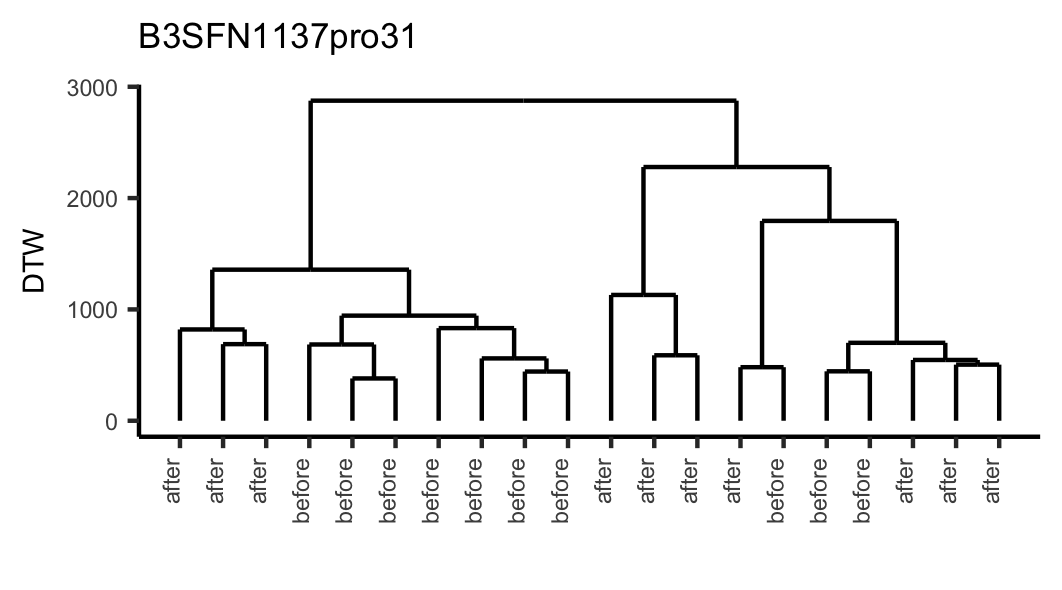
\includegraphics[width=15cm]{fig/dendro_4.png}
		\caption{デンドログラム4}
		\label{fig:dendro4}
	\end{center}
\end{figure}
\begin{figure}[H]
	\begin{center}
		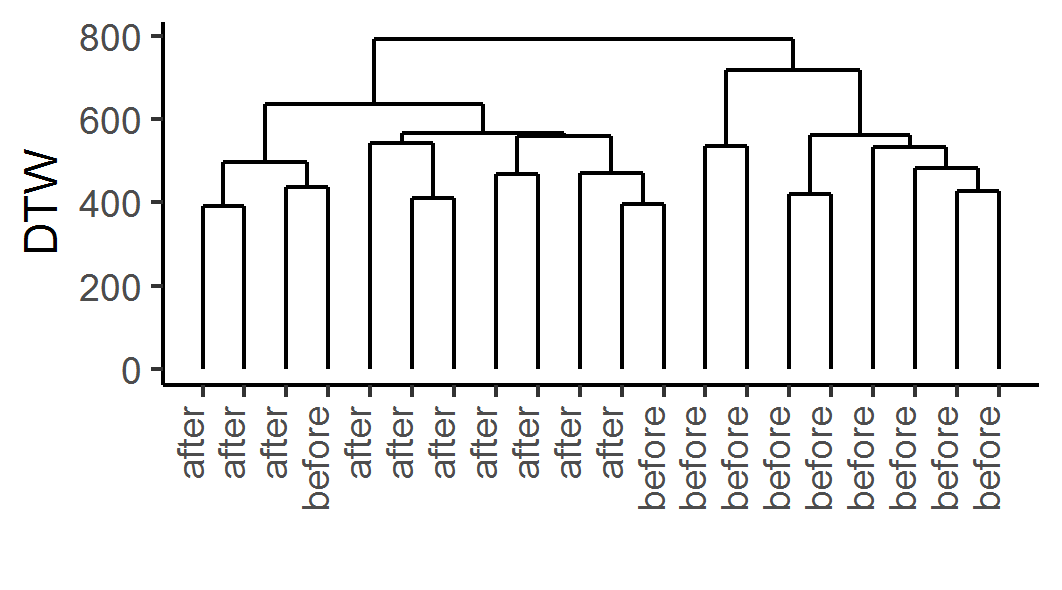
\includegraphics[width=15cm]{fig/dendro_5.png}
		\caption{デンドログラム5}
		\label{fig:dendro5}
	\end{center}
\end{figure}
\begin{figure}[H]
	\begin{center}
		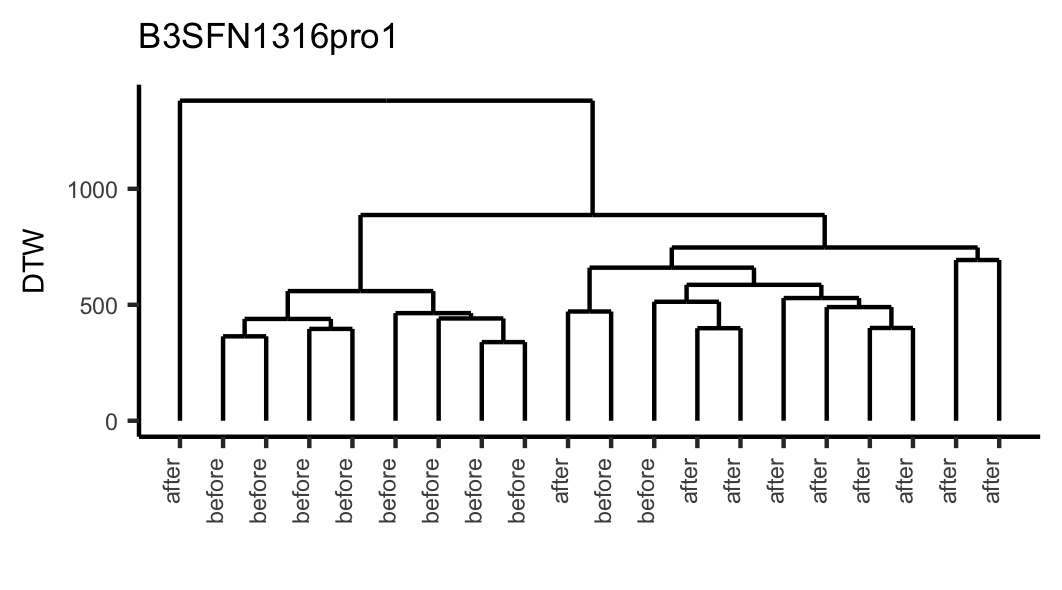
\includegraphics[width=15cm]{fig/dendro_6.png}
		\caption{デンドログラム6}
		\label{fig:dendro6}
	\end{center}
\end{figure}
\begin{figure}[H]
	\begin{center}
		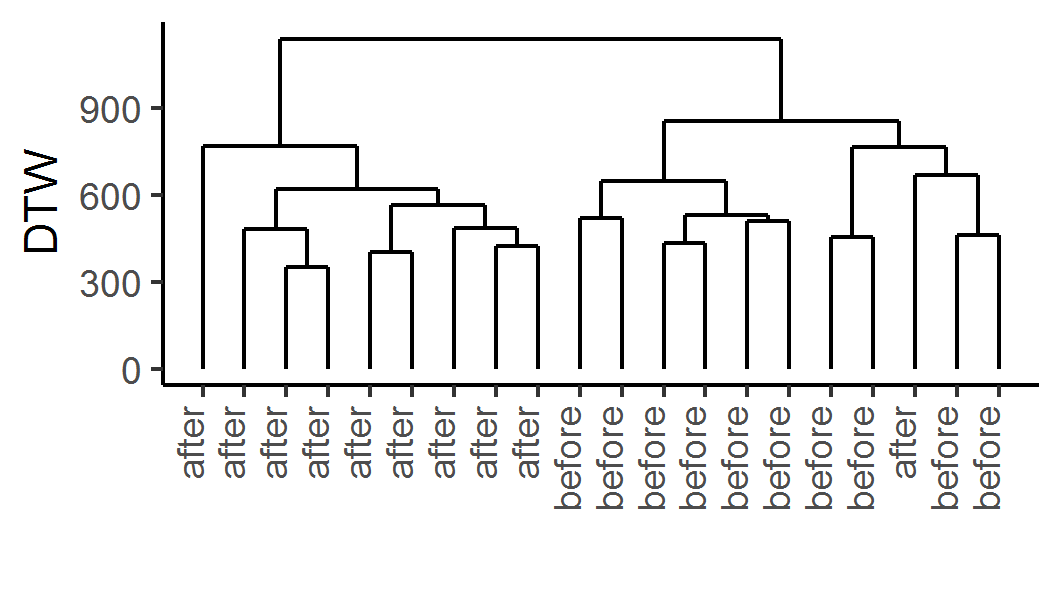
\includegraphics[width=15cm]{fig/dendro_7.png}
		\caption{デンドログラム7}
		\label{fig:dendro7}
	\end{center}
\end{figure}
\begin{figure}[H]
	\begin{center}
		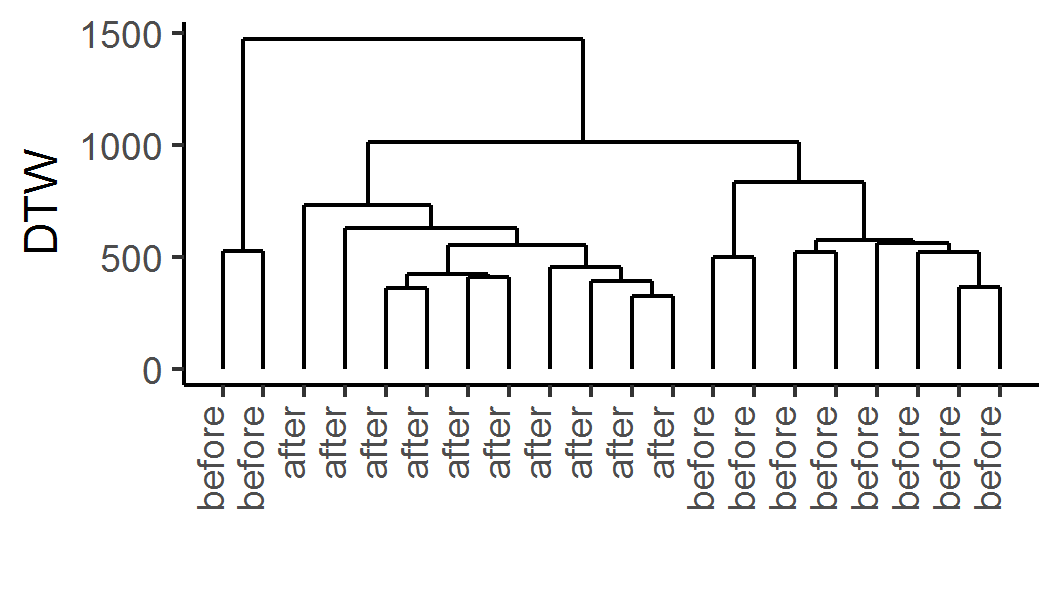
\includegraphics[width=15cm]{fig/dendro_8.png}
		\caption{デンドログラム8}
		\label{fig:dendro8}
	\end{center}
\end{figure}
\begin{figure}[H]
	\begin{center}
		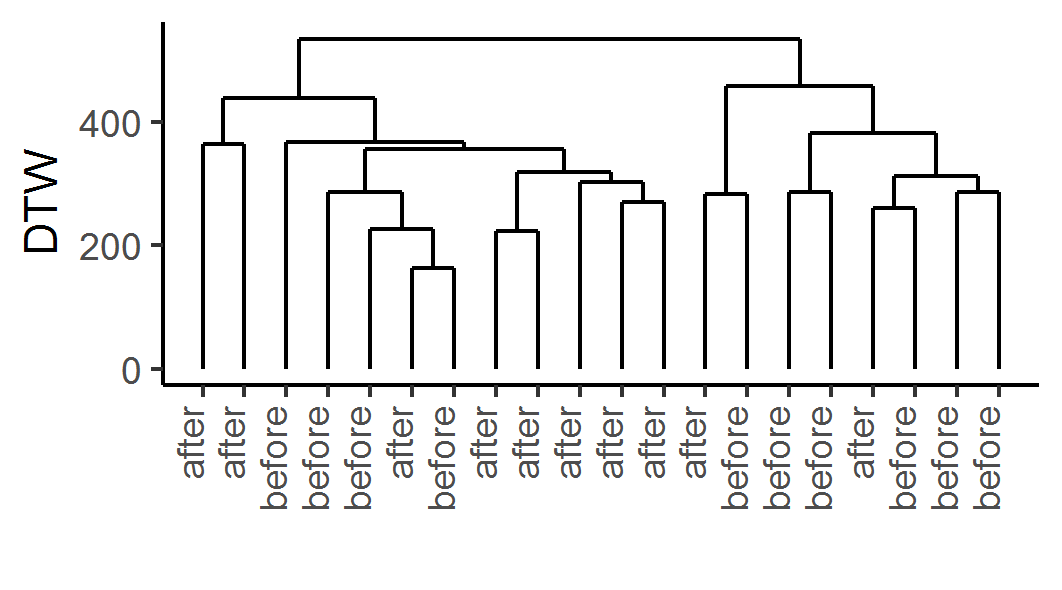
\includegraphics[width=15cm]{fig/dendro_9.png}
		\caption{デンドログラム9}
		\label{fig:dendro9}
	\end{center}
\end{figure}
\begin{figure}[H]
	\begin{center}
		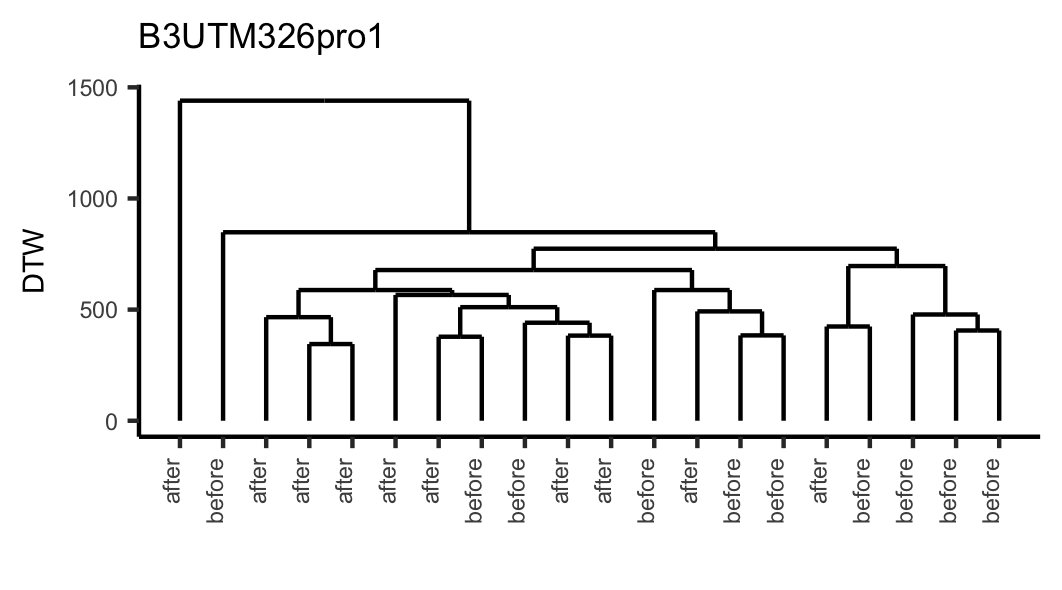
\includegraphics[width=15cm]{fig/dendro_10.png}
		\caption{デンドログラム10}
		\label{fig:dendro10}
	\end{center}
\end{figure}
\begin{figure}[H]
	\begin{center}
		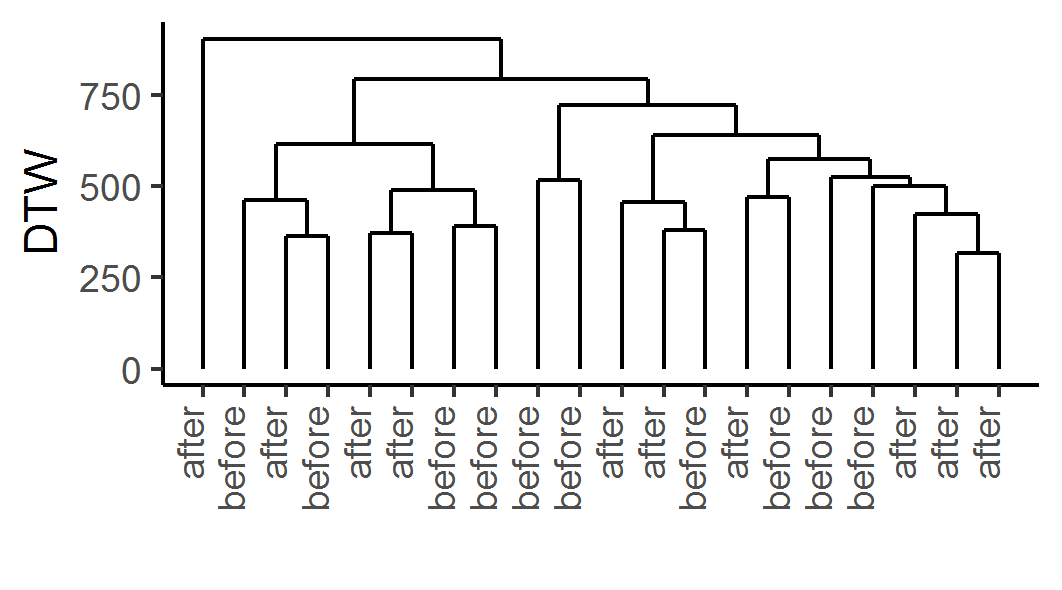
\includegraphics[width=15cm]{fig/dendro_11.png}
		\caption{デンドログラム11}
		\label{fig:dendro11}
	\end{center}
\end{figure}
\begin{figure}[H]
	\begin{center}
		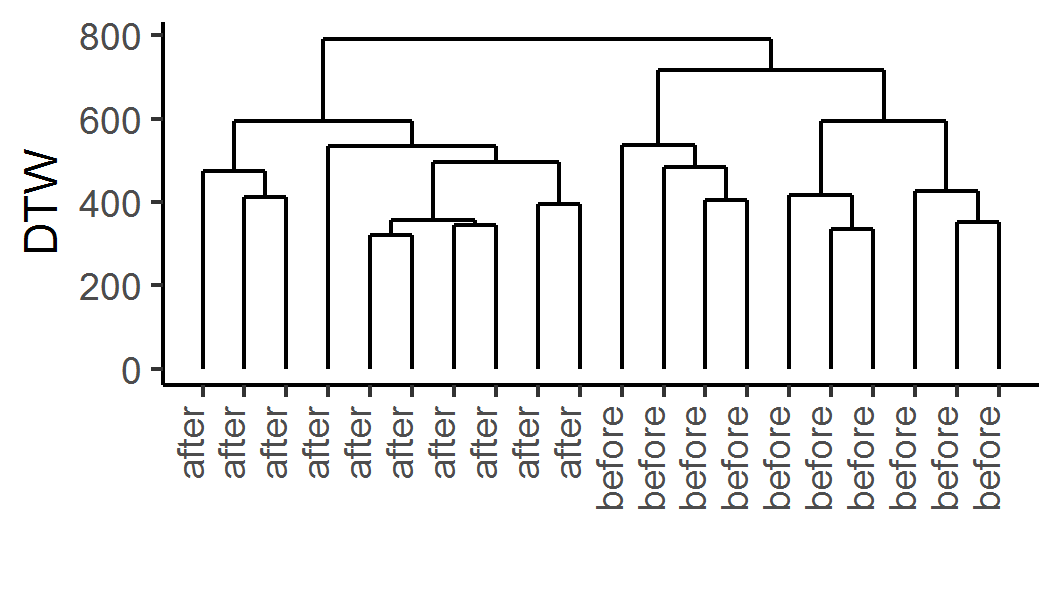
\includegraphics[width=15cm]{fig/dendro_12.png}
		\caption{デンドログラム12}
		\label{fig:dendro12}
	\end{center}
\end{figure}
\begin{figure}[H]
	\begin{center}
		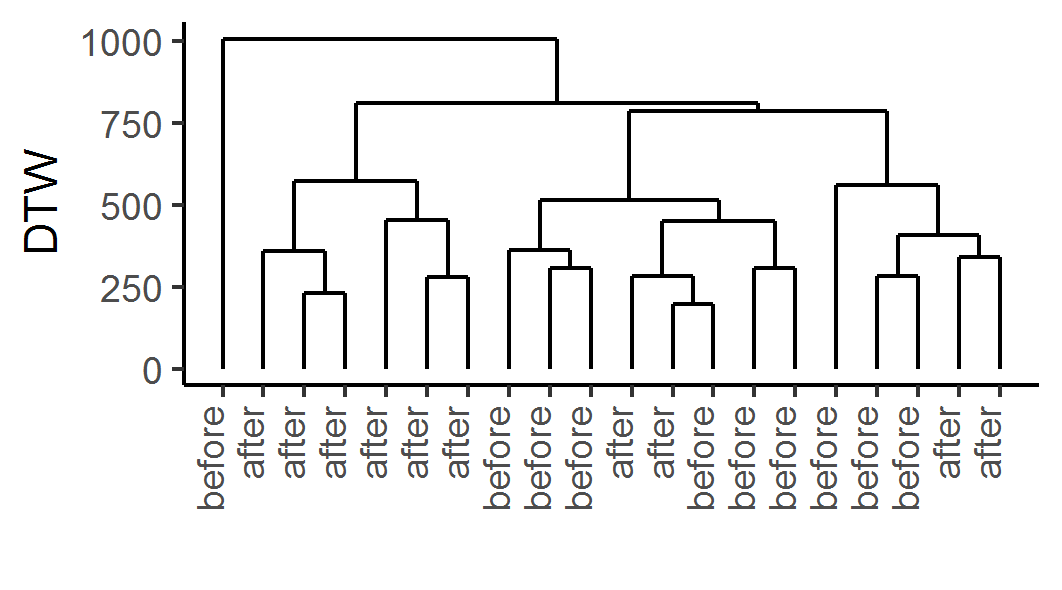
\includegraphics[width=15cm]{fig/dendro_13.png}
		\caption{デンドログラム13}
		\label{fig:dendro13}
	\end{center}
\end{figure}
\begin{figure}[H]
	\begin{center}
		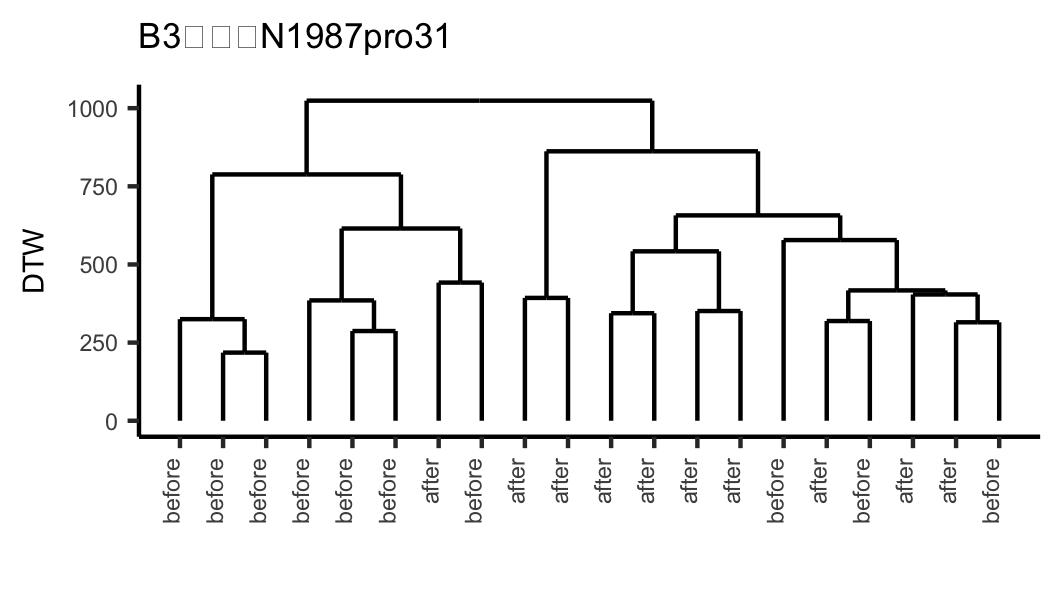
\includegraphics[width=15cm]{fig/dendro_14.png}
		\caption{デンドログラム14}
		\label{fig:dendro14}
	\end{center}
\end{figure}
\begin{figure}[H]
	\begin{center}
		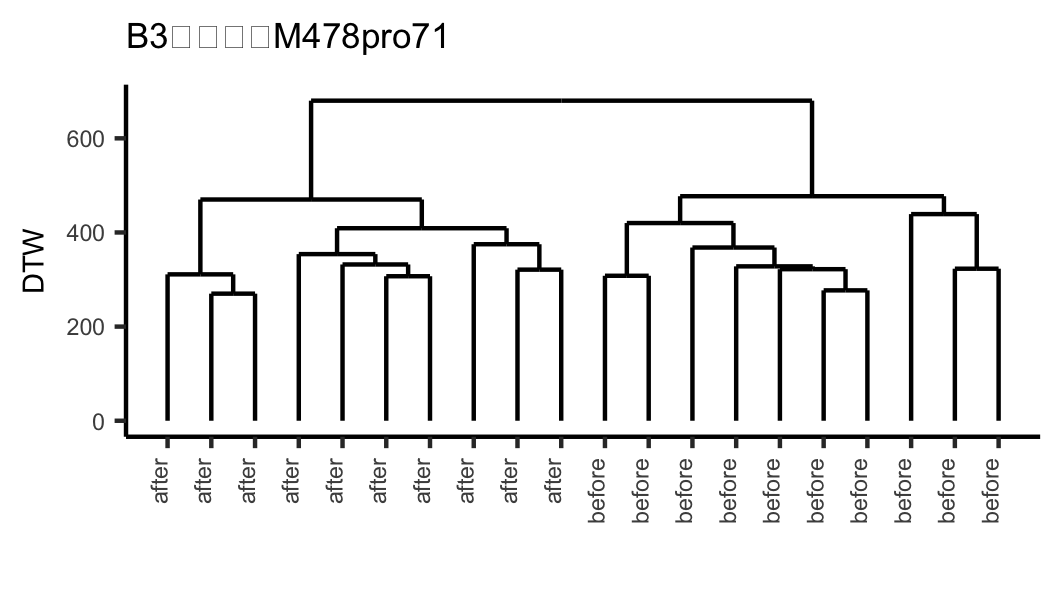
\includegraphics[width=15cm]{fig/dendro_15.png}
		\caption{デンドログラム15}
		\label{fig:dendro15}

	\end{center}
\end{figure}



\section{考察・今後の課題}






\bibliography{TDA} %hoge.bibから拡張子を外した名前


\end{document}